\section{Optimizer Selection and Tuning}
\subsection{SGD}
Standard SGD updates parameters with the current minibatch gradient. The
baseline uses learning rate 0.01 and no momentum.
\subsection{SGD with Momentum}
Momentum accumulates a velocity from earlier gradients; this can accelerate
consistent descent directions \cite{sutskever2013}. The experiment uses
learning rate 0.01 and momentum 0.9, without Nesterov acceleration.
For minibatch gradient $g_t$, the update can be written as
\begin{equation}
v_t=\mu v_{t-1}+g_t,\qquad
\theta_{t+1}=\theta_t-\eta v_t,
\label{eq:momentum}
\end{equation}
where $\eta$ is the learning rate and $\mu$ is the momentum coefficient.
Equation~\eqref{eq:momentum} reduces to standard SGD when $\mu=0$.
Accumulating gradients can smooth inconsistent directions, although it does
not guarantee a smoother validation curve.
\subsection{Adam}
Adam adapts updates using first and second gradient moments \cite{kingma2015}.
The tested learning rate is 0.001, with default betas $(0.9,0.999)$ and
$\epsilon=10^{-8}$.
\subsection{Experimental Comparison}
Model B is used for its low compute requirement. Each recipe uses ten epochs,
batch size 128, identical initial weights, seed, data order and augmentation
strategy. No weight decay, scheduler or early stopping is used. These are
controlled recipe comparisons, not exhaustive learning-rate searches.
Table~\ref{tab:optimizers} records settings, best validation performance and
final validation accuracy; Table~\ref{tab:optimizer_dynamics} adds final losses
and timing. ``Final'' here means the last pilot epoch, not a test-set result.
The pilot test sets are not evaluated for optimizer selection.
% Generated from saved experiment evidence; do not edit values.
\begin{table}[H]\centering\small
\caption{Optimizer comparison on Model B; each run uses ten epochs. Adam moment coefficients are specified in the text.}\label{tab:optimizers}
\begin{tabular}{lrrrrr}
\toprule
Optimizer & LR & Momentum & Best val. (\%) & Epoch & Final val. (\%) \\ \midrule
Adam & 0.001 & -- & 91.46 & 10 & 91.46 \\
SGD + momentum & 0.01 & 0.9 & 90.57 & 8 & 90.52 \\
SGD & 0.01 & 0 & 81.63 & 9 & 80.05 \\
\bottomrule
\end{tabular}
\end{table}

% Generated from saved experiment evidence; do not edit values.
\begin{table}[H]\centering\small
\caption{Final-epoch optimizer losses and training accuracy; mean timing spans all ten epochs.}\label{tab:optimizer_dynamics}
\begin{tabular}{lrrrr}
\toprule
Optimizer & Train loss & Val. loss & Train acc. (\%) & Epoch (s) \\ \midrule
SGD & 0.545 & 0.573 & 81.52 & 3.164 \\
SGD + momentum & 0.250 & 0.277 & 91.35 & 2.963 \\
Adam & 0.220 & 0.246 & 92.30 & 3.078 \\
\bottomrule
\end{tabular}
\end{table}

Figure~\ref{fig:optimizer_comparison} shows that plain SGD improves gradually
but finishes with higher validation loss than the other recipes. Momentum
reaches a much higher validation accuracy within the same budget, despite
fluctuations during the middle epochs. Adam finishes with the lowest validation
loss, \AdamPilotFinalLoss{}, compared with \MomentumPilotFinalLoss{} for
momentum SGD and \SgdPilotFinalLoss{} for plain SGD.
\begin{figure}[H]\centering
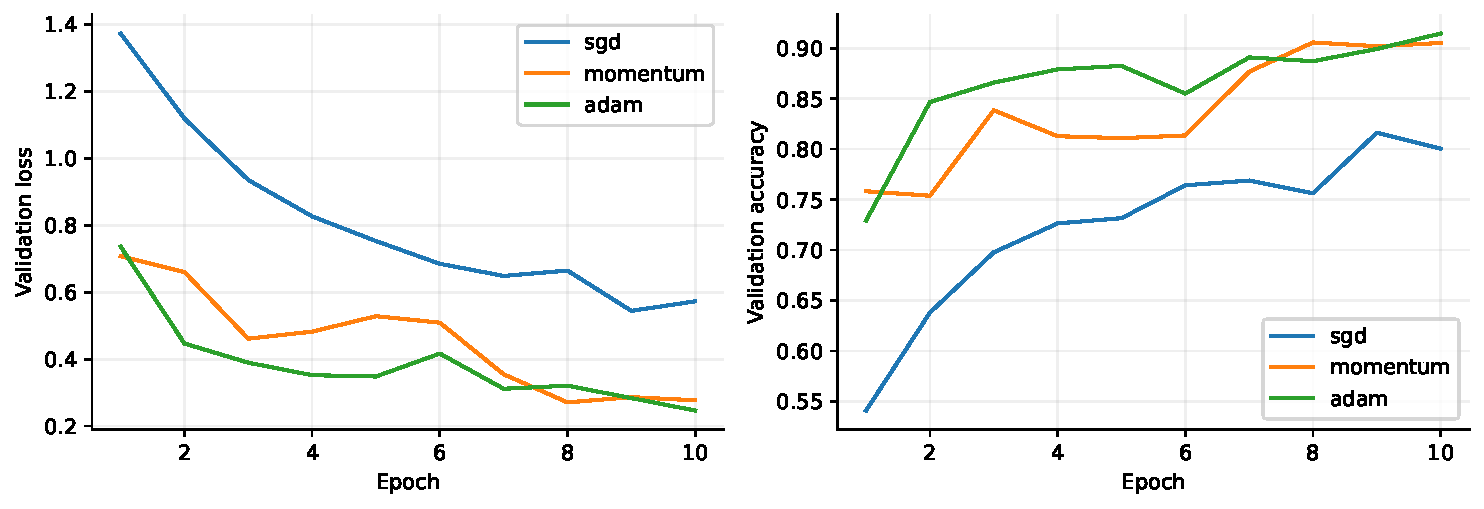
\includegraphics[width=0.96\textwidth]{figures/optimizer_comparison.pdf}
\caption{Validation loss and accuracy; unsmoothed observations.}
\label{fig:optimizer_comparison}
\end{figure}
\subsection{Selected Optimizer}
Adam is selected by highest validation accuracy, with lower validation loss
breaking ties. Its best validation accuracy is \AdamPilotBest\%, compared with
\MomentumPilotBest\% for momentum SGD and \SgdPilotBest\% for plain SGD.
Momentum therefore improves on plain SGD by \MomentumGain{} percentage points
at the same learning rate. Adam's advantage over momentum SGD is smaller,
\AdamMomentumGap{} percentage points, and also involves a different learning
rate. This experiment supports choosing Adam for the final runs; it does not
isolate optimizer type from learning-rate choice or establish universal
superiority. Losses are still improving near the end, so the fixed budget does
not establish full convergence. The initial settings were retained, and no
setting was chosen using test performance.
